
\iffalse


\title{assignment}
\author{EE24BTECH11020}
\section{integer}
\fi


\item The number of times digit 3 will be written when listing the integers from 1 to 1000 is \underline{\hspace{1cm}}\hfill (March 2021)
\\ 
\item The equation of the planes parallel to the plane $x - 2y + 2z - 3 = 0$ which are at unit distance from the point $\brak{1, 2, 3}$ is $ax + by + cz + d = 0$. If $\brak{b - d} = K\brak{c - a}$, then the positive value of $K$ is \underline{\hspace{1cm}}\hfill (March 2021)
\\
\item Let $f\brak{x}$ and $g\brak{x}$ be two functions satisfying $f\brak{x^2} + g\brak{4 - x} = 4x^3$ and $g\brak{4 - x} + g\brak{x} = 0$, then the value of $\int_{-4}^{4} f(x^2) \, dx$ is \underline{\hspace{1cm}}\hfill (March 2021)
\\
\item The mean age of 25 teachers in a school is 40 years. A teacher retires at the age of 60 years and a new teacher is appointed in his place. If the mean age of the teachers in this school now is 39 years, then the age (in years) of the newly appointed teacher is \underline{\hspace{1cm}}\hfill (March 2021)
\\

\item A square $ABCD$ has all its vertices on the curve $x^2y^2 = 1$. The midpoints of its sides also lie on the same curve. Then, the square of the area of $ABCD$ is \underline{\hspace{1cm}}\hfill (March 2021)
\\
\item The missing value in the following figure is \underline{\hspace{1cm}}\hfill (March 2021)



 \begin{center}
     

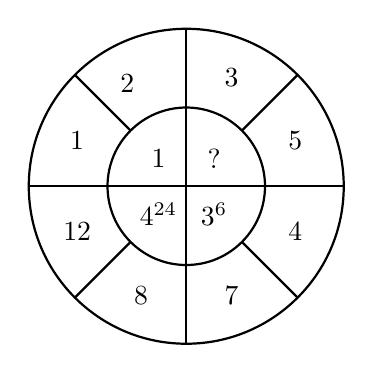
\begin{tikzpicture}


\draw[thick, black] (0, 0) circle (2);


\draw[thick, black] (0, 0) circle (1);



\draw[thick, black] (0, 0) -- (0:2);
\draw[thick, black] (0, 0) -- (90:2);
\draw[thick, black] (0, 0) -- (180:2);
\draw[thick, black] (0, 0) -- (270:2);

\node at (157.5:1.5) {1};
\node at (120:1.5) {2};
\node at (67.5:1.5) {3};
\node at (22.5:1.5) {5};
\node at (-22.5:1.5) {4};
\node at (-67.5:1.5) {7};

\node at (-112.5:1.5) {8};
\node at (-157.5:1.5) {12};


\node at (-135:0.5) {$4^{24}$};
\node at (-45:0.5) {$3^6$};
\node at (135:0.5) {1};
\node at (45:0.5) {?};
\draw[thick,black] (45:2) -- (45:1);
\draw[thick,black] (135:2) -- (135:1);
\draw[thick,black] (-135:2) -- (-135:1);
\draw[thick,black] (-45:2) -- (-45:1);


\end{tikzpicture}   \end{center}   

\item Let $z_1, z_2$ be the roots of the equation $z^2 + az + 12 = 0$ and $z_1, z_2$ form an equilateral triangle with the origin. Then, the value of $\abs{a}$ is \underline{\hspace{1cm}}.\hfill (March 2021)
\\

\item The number of solutions of the equation $\abs{\cot x}  = \cot x + \frac{1}{\sin x}$ in the interval \sbrak{0, 2\pi} is \underline{\hspace{1cm}}\hfill (March 2021)
\\

\item Let the plane $ax + by + cz + d = 0$ bisect the line joining the points $\brak{4, -3, 1}$ and $\brak{2, 3, -5}$ at right angles. If $a, b, c, d$ are integers, then the minimum value of $\brak{a^2 + b^2 + c^2 + d^2}$ is \underline{\hspace{1cm}}. \hfill (March 2021)
\\
\item If $f(x) = \int \frac{5x^8 + 7x^6}{(x^2 + 1 + 2x^7)^2} \, dx$, $\brak{x \geq 0}$, $f(0) = 0$ and $f(1) = \frac{1}{k}$, then the value of $k$ is \underline{\hspace{1cm}}\hfill (March 2021)
